\documentclass{report}
\usepackage{graphicx}
\usepackage{listings}
\usepackage{xcolor}
\usepackage{array}
\usepackage[a4paper, total={6in, 10in}]{geometry}
\usepackage{amssymb}
\usepackage{amsmath}
\usepackage{tikz}


\definecolor{codegreen}{rgb}{0,0.6,0}
\definecolor{codegray}{rgb}{0.5,0.5,0.5}
\definecolor{codepurple}{rgb}{0.58,0,0.82}
\definecolor{backcolour}{rgb}{0.95,0.95,0.92}

\lstdefinestyle{mystyle}{
	backgroundcolor=\color{backcolour},   
	commentstyle=\color{codegreen},
	keywordstyle=\color{magenta},
	numberstyle=\tiny\color{codegray},
	stringstyle=\color{codepurple},
	basicstyle=\ttfamily\footnotesize,
	breakatwhitespace=false,         
	breaklines=true,                 
	captionpos=b,                    
	keepspaces=true,                 
	numbers=left,                    
	numbersep=5pt,                  
	showspaces=false,                
	showstringspaces=false,
	showtabs=false,                  
	tabsize=2
}
\lstset{style=mystyle}
\graphicspath{ {images/} }
\title{Design II\\ HoGent}
\author{JeeVeeVee}
\date{2020/2021}
\begin{document}
	\maketitle
   	\tableofcontents
   	\chapter{Factory pattern}
   		The principle of a factory is that you take the code for creating an object, and move it to another object which will have as single responsibility creating these objects. 
   		\section{Simple Factory}
   			Often works with a simple switch statement. The factory has a client who 'orders' the object from the factory. The create-method is often static.
   		\section{Factory Method}
   			There is an abstract class with an abstract method, the factory method. The sub-classes implement this factory method, this way, you don't have to outsource the creation of the objects. The sub-classes decide how the method is implemented. In this case, the class hierarchies are parallel : both contain abstract classes which are extended into concrete classes which contain specific implementations.
   			\begin{center}
   				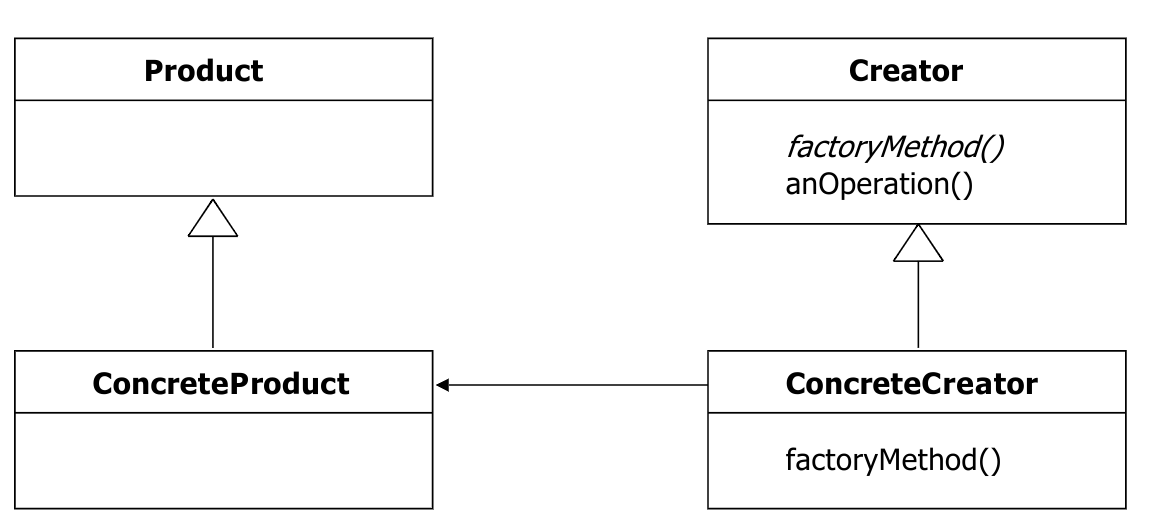
\includegraphics[scale=0.3]{factory_method}
   			\end{center}
   			The factory method relies on the \textbf{dependency inversion principle} which states that it is beter to be dependent on abstractions rather then to be dependent on concrete classes.
   			\pagebreak
   		\section{Abstract Factory}
   			An abstract factory supplies an interface for a set of products. The code is designed so that we use a factory to create the products, this way the client code stays the same, we do get multiple implementations of our products.
   			\begin{center}
   				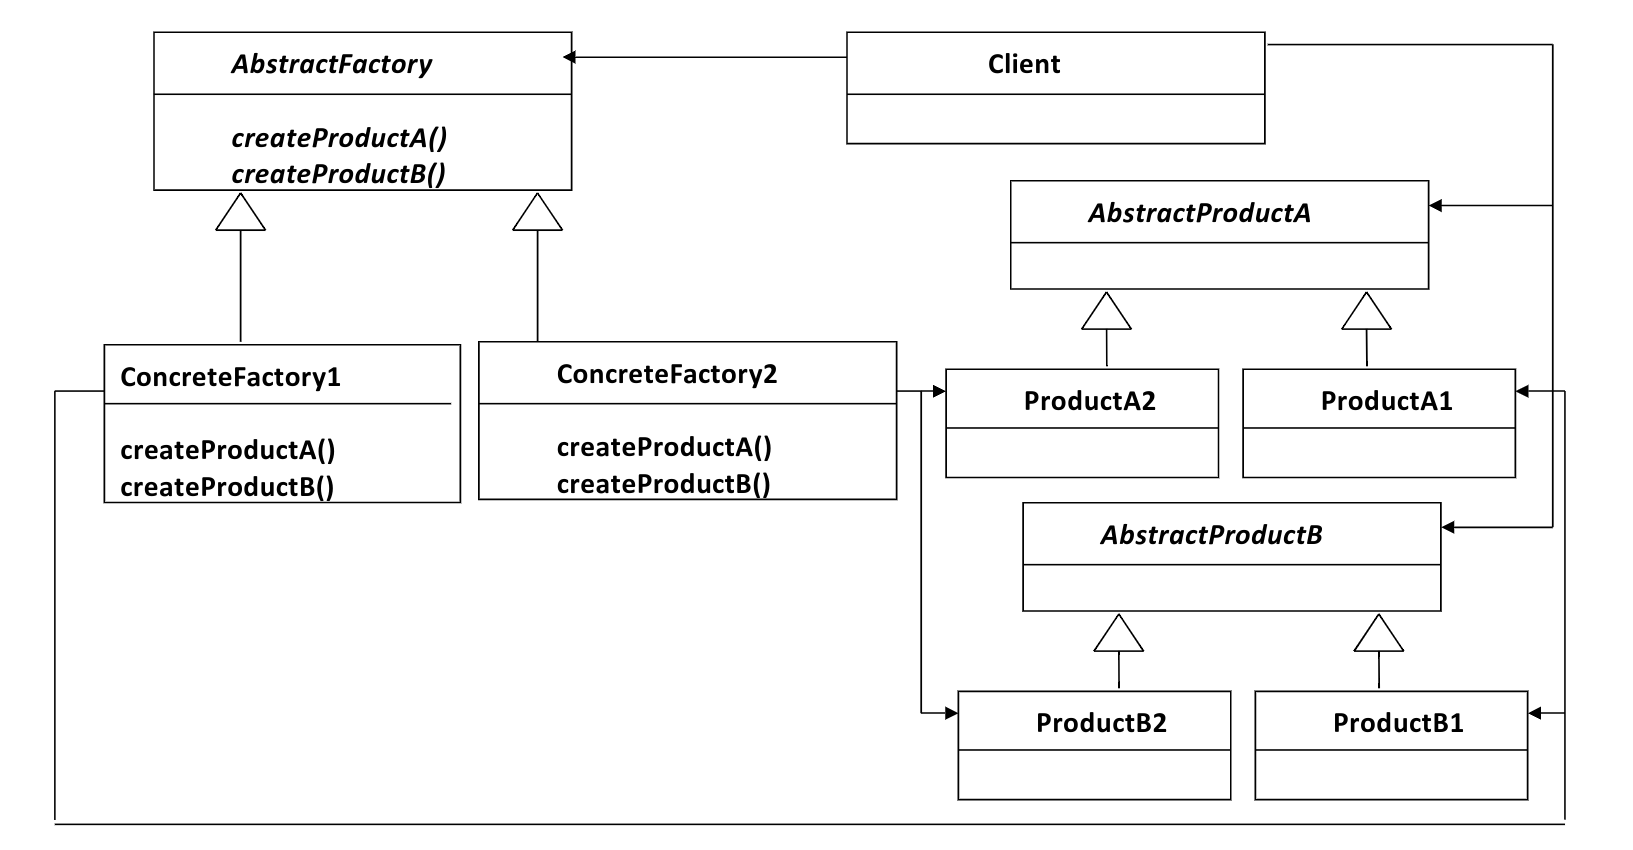
\includegraphics[scale=0.3]{abstract_factory}
   			\end{center}
   	\chapter{Iterator and Composite pattern}
   		\section{Iterator patters}
   			You want the client to access 2 different implementations with the same functionality. To achieve this, you have to create some kind of translator in the middle who can communicate with both of the implementations. This way the differences in implementation are invisible to the client. The iterator pattern feels a lot like a facade...
   			\begin{center}
   				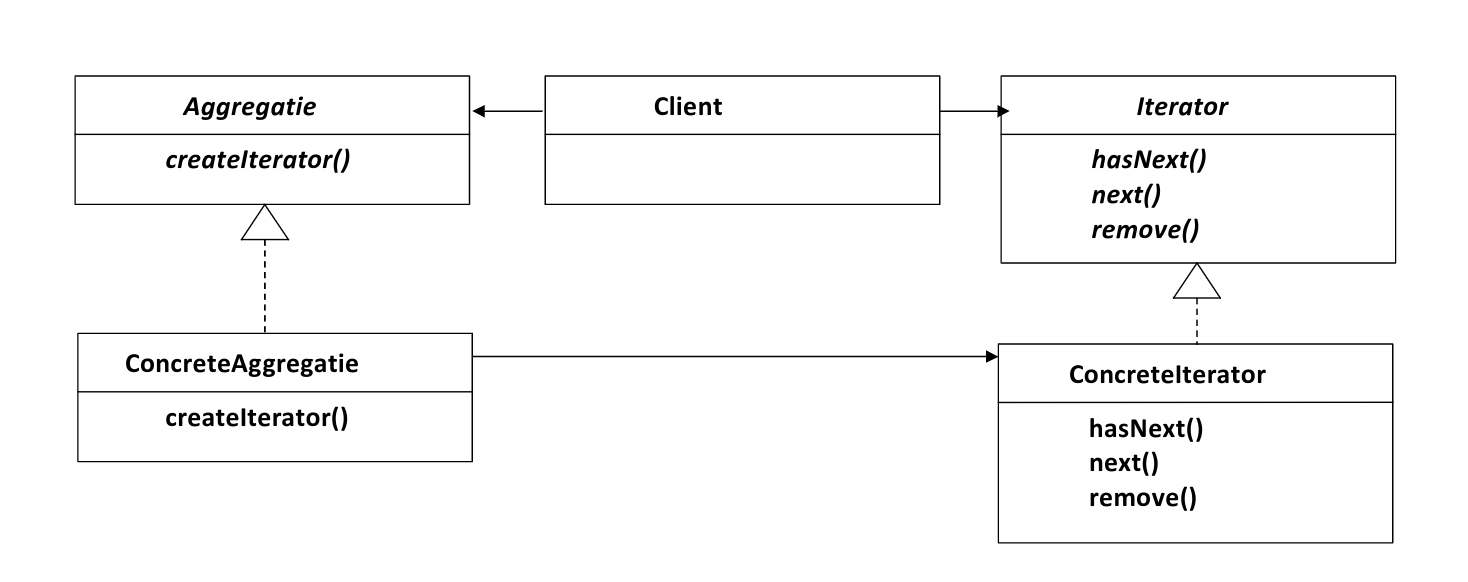
\includegraphics[scale=0.3]{iterator}
   			\end{center}
   			The iterator pattern is build on the \textbf{single responsibility principle} which states that there should only reason for a class to change.
   			\pagebreak
   		\section{Composite Pattern}
   			The composite patters allows you to represent a part-whole hierarchy as a tree structure, enabling you to process individual objects or a group of objects in a uniform way. In short, the composite allows us to represent the following situation : 
   			\begin{center}
   				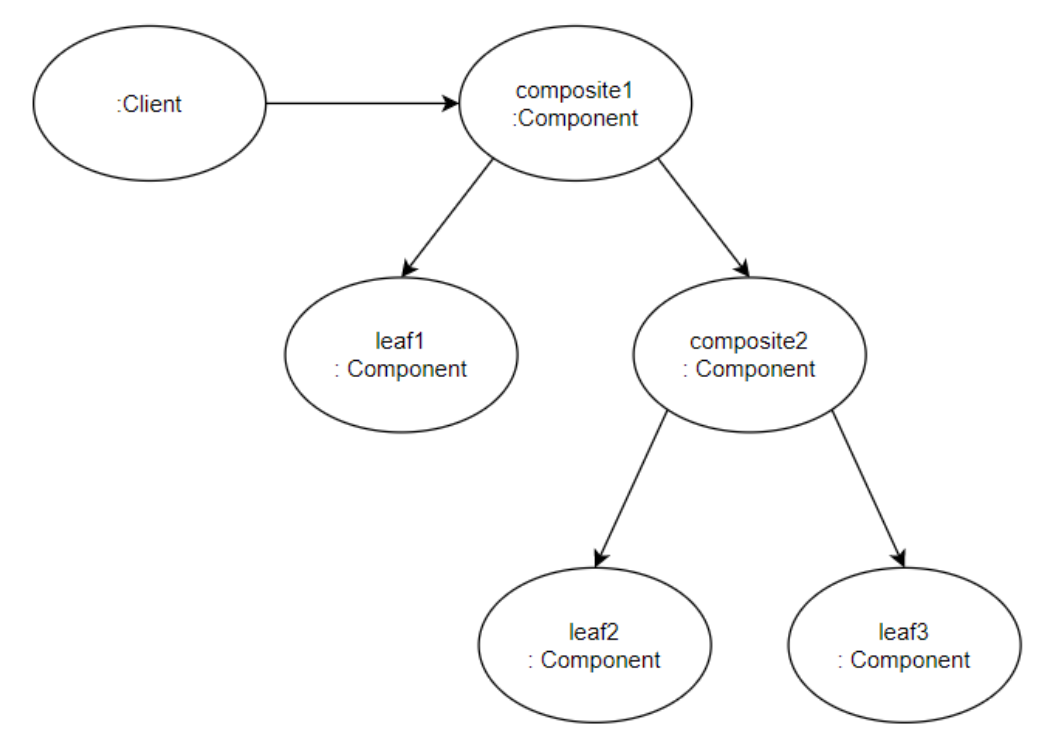
\includegraphics[scale=0.3]{composite_irl}
   			\end{center} 
   			By this UML: 
   			\begin{center}
   				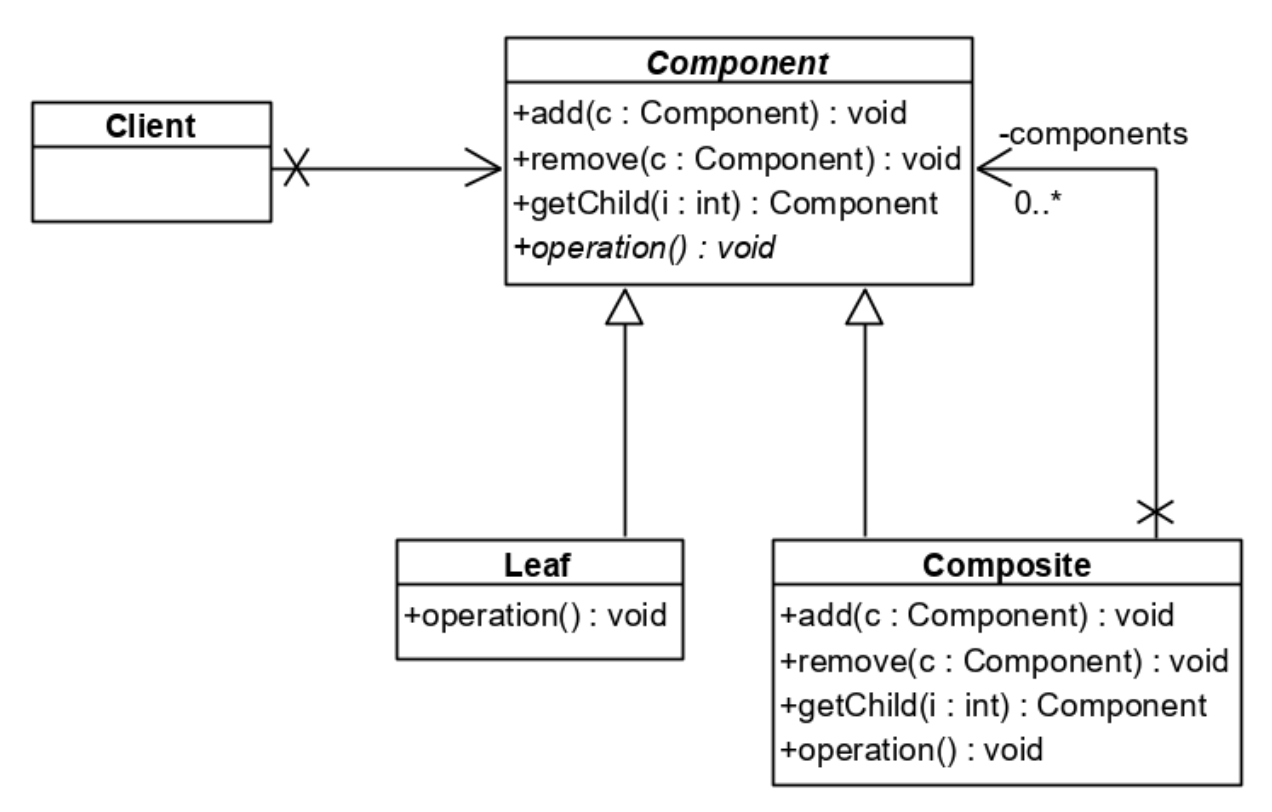
\includegraphics[scale=0.3]{composite_uml}
   			\end{center} 
   			The Composite defines the behavior of components with child components and contains children. The Leaf defines the behavior of elements in the hierarchy, it has no children. The Component is the interface for objects in the hierarchy. This does mean that some methods in both Leaf and Composite will throw UnsupportedException since they don't makes sense otherwise.
	\chapter{Builder}
		The builder pattern is used to encapsulate (hide) the construction logic, allowing for complex objects to be constructed in incremental steps. Some classes have lot of options and multiple constructors, you could solve this by using setters, but this doesn't guarantee the correct order which is sometimes pretty important. Another solution is a Builder class, this way we can define a fixed order of steps, disadvantage of this method is that we can only build 1 specific type of object (the one with that particular order). To make our design more flexible, we need a flexible data structure which can represent different objects. We can achieve this flexibility by using an Iterator.
   		\begin{center}
   			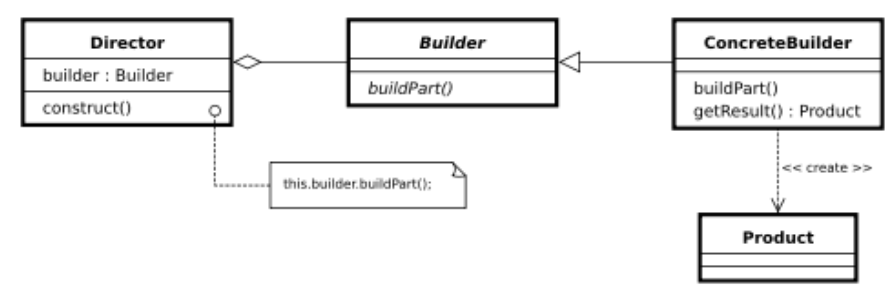
\includegraphics[scale=0.5]{builder}
   		\end{center} 
   		The Builder class specifies an abstract interface for creating parts of the Product object. The Concrete Builder implements the Builder interface. The Director class builds the complex object, using a Builder interface. Product represents the complex object that is being built.
   		The advantages are : 
   		\begin{itemize}
   			\item encapsulates how a complex object is being built 
   			\item allows for creating an object in multiple steps, where there is only 1 step if you use a factory.
   			\item hides the internal representation of the product form the client
   			\item the product implementations can change at all times since the client only accesses the abstract interface it implements.
   		\end{itemize}
	\chapter{Command Pattern}
		The Command pattern encapsulates a request as an object, thereby letting you parameterize other object with different requests, queue or log requests, and support undoable operations. 
   		\begin{center}
   			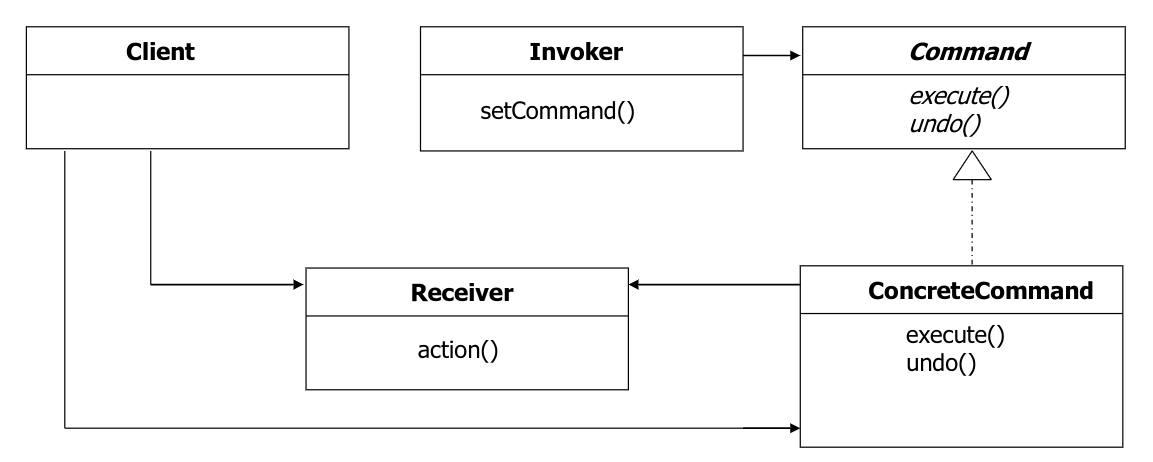
\includegraphics[scale=0.4]{command}
   		\end{center} 
   		The Client is responsible for creating a ConcreteCommand, The receiver knows how to preform the work needed to carry out the request, this could be any class. The Invoker holds the command and at some point, it will ask the command to carry out a request by calling the .execute() method.
   		\\
   		The Command pattern decouples an object making a request from the one that knows how to preform it. This pattern feels a lot like State...
   	\chapter{Template Method Pattern}
   		The Template Method Pattern defines the skeleton of an algoritm in a method, leaving some steps to subclasses. The pattern relies on subclasses to define some steps of an algoritm without allowing them to change the general structure of the algoritm(because the templateMethod is final). 
   		\begin{center}
   			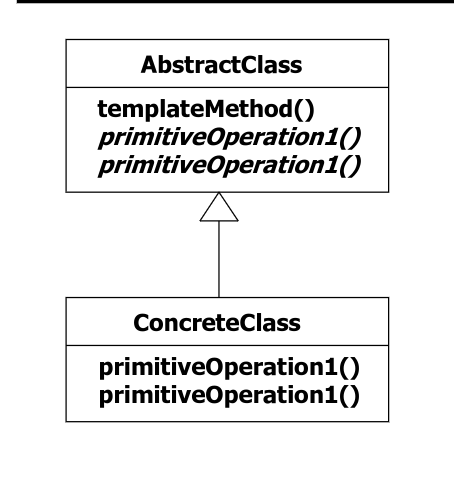
\includegraphics[scale=0.6]{template_method}
   		\end{center} 
   		You can use a hook to overwrite a method, if you would want to. 
   		\\
   		This pattern uses the \textbf{Hollywood principle} which states "Don't call us, we'll call you". This mean the high-level component decides when and how the low-level component participates, a low-level component however, never invokes a high-level component.
	\chapter{Adapter}
		An Adapter is used to link an existing system to library classes.This way Adapter allows classes to work together even if they have incompatible interfaces.
		\begin{center}
			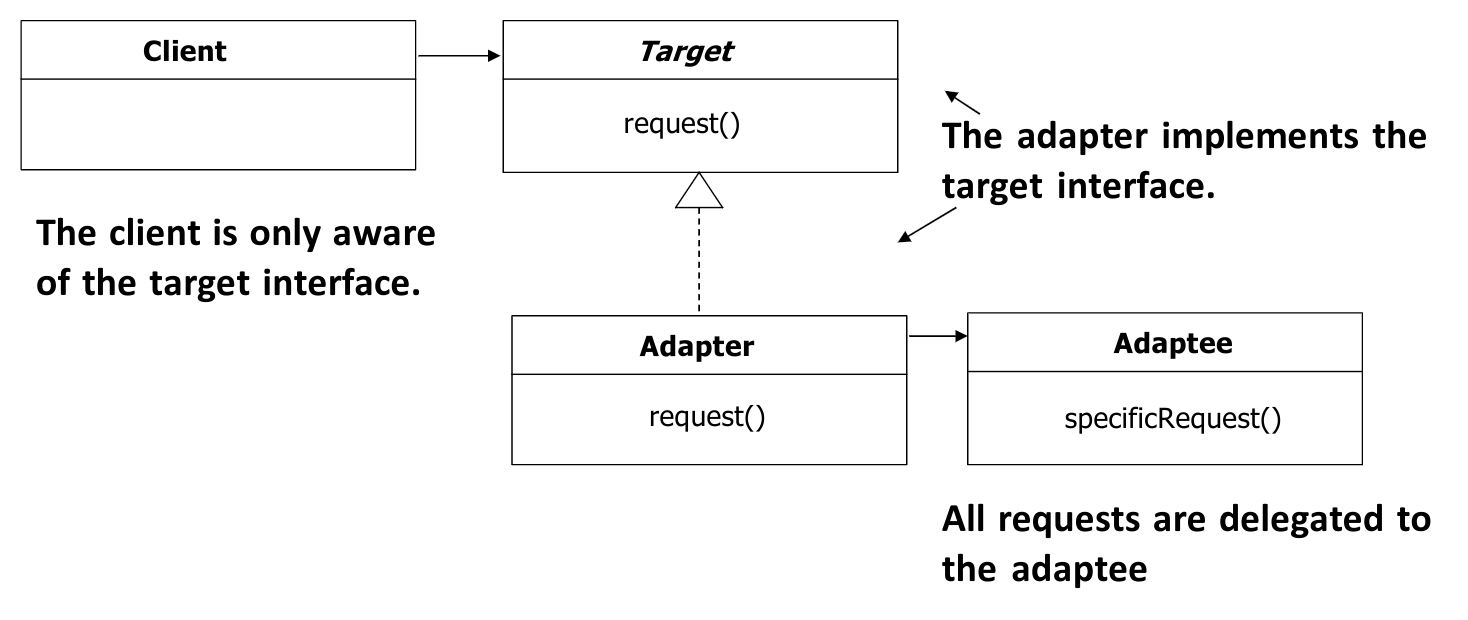
\includegraphics[scale=0.3]{adapter}
		\end{center}
	\chapter{Proxy} 
		It is a structural design pattern, it allows you to replace another object, it will give or deny you control over that object. 
		\section{Remote Proxy}
			A remote proxy acts as a local representation of a remote object. The original object runs in a different JVM. The proxy contains a set of local methods which can be called and which are then transferred to the remote object. 
			\subsection{RMI (Remote Method Invocation)}
				By adding a client helper and a service helper, the client will feel like he is interacting with the real deal, while in fact the client helper is a proxy which acts as a real thing, but transfers all operations to the original object. \\
				The following steps are taken when an method is called:
				\begin{enumerate}
					\item The client object calls the method doBigThing() of the client helper object
					\item The client helper object wraps all the info and transfers it over the network to the service helper.
					\item The service helper now needs to unwrap the info and can call the real method on the real service object.
					\item The service object does al the work and returns the result to the service helper.
					\item The service helper wraps all the results and sends it over the network to the client helper
					\item the client helper now unwraps the result and returns it to the client object who doesn't know what just happend
				\end{enumerate}
			\begin{center}
				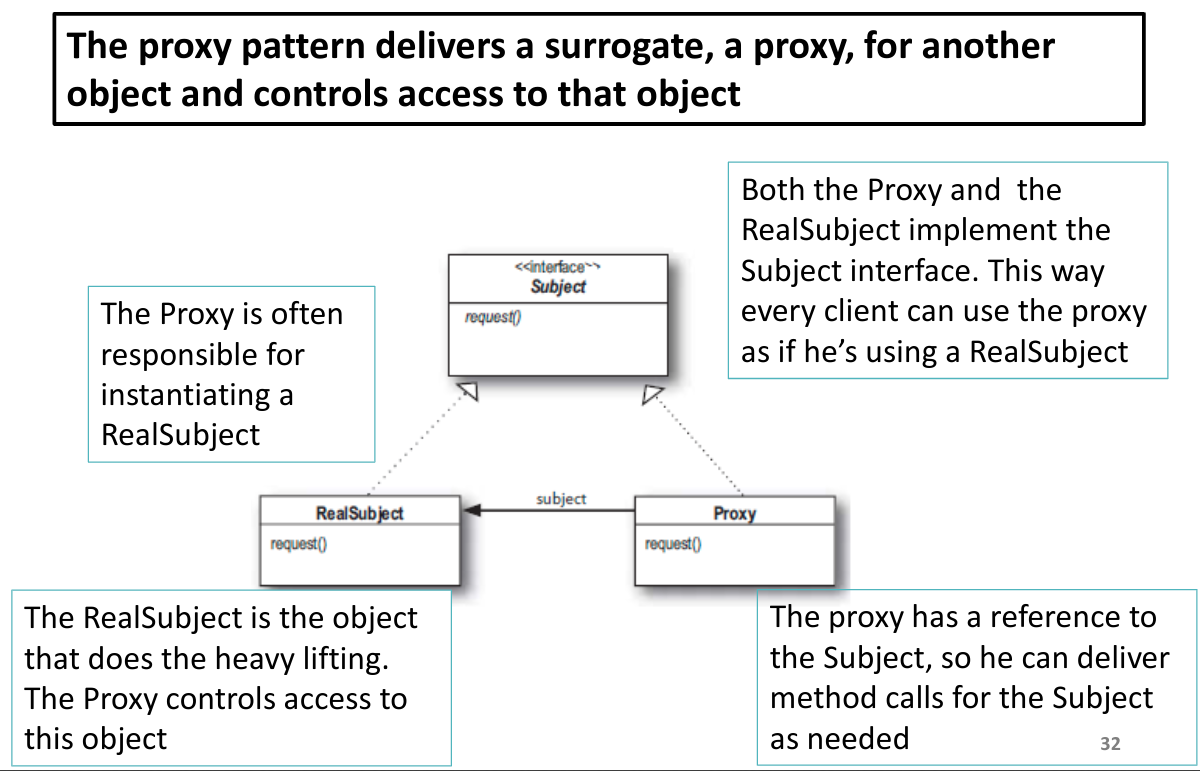
\includegraphics[scale=0.4]{remote_proxy}
			\end{center}
		\section{Virtual proxy}
			A virtual proxy represents an object that is way too expensive to create. the proxy acts as a surrogate for the object when created. Other methods are delegated to the realSubject.
			\subsection{Protection}
				We can use Java's proxy API to add protection. Instead of the proxy having a reference to RealSubject, he now has a reference to InvocationHandler, which does have a reference to RealSubject. The proxy now exists out of 2 classes. The invocationHandler is now in charge of restricting access to the realsubject. This is different from a decorator as a decorator adds behaviour to an object, where proxy controls access.
	\chapter{Singleton}
		Sometimes we have objects of which only 1 instance is needed/wanted. A singleton guarantees one and only instance of a class exits in you program. It serves as a global access to the instance and is created as needed.
		\begin{lstlisting}[language = java]
public class Singelton{
	private static final Singleton uniqueInstance = new Singleton();
	
	//nuttige variabelen
	
	private Sinlgeton(){
	}
	
	public static Singleton getInstance(){
		return uniqueInstance;
	}
}\end{lstlisting}
		\section{lazy loading}
			Lazy loading is a design pattern commonly used in computer programming to defer initialization of an object until the point at which it is needed. It can contribute to efficiency in the program's operation if properly and appopriately used. The opposite is called eager loading. You can make an Singleton lazy by adding some code to the getInstance method.
			\begin{lstlisting}[language = java]
public class Singelton{
private static final Singleton uniqueInstance;

//nuttige variabelen

private Sinlgeton(){
}

public static Singleton getInstance(){
	if(uniqueInstance = null){
		uniqueInstance = new Singleton
	}
	return uniqueInstance;
}\end{lstlisting}
			\section{Multithreading}
				When using lazy loading, in combination with multithreading, it is possible that there will be more then 1 instance of the Singleton. It is safer to then work with eager loading (= creating an instance when the class is loaded). 
				If you still want to use lazy loading, you will have to make the getInstance() method synchronized, this will possibly reduce performace a lot!!!
		
\end{document}